\documentclass[10pt]{article}
\usepackage[letterpaper,margin=0.78in]{geometry}
\usepackage[T1]{fontenc}
\usepackage[utf8]{inputenc}
\usepackage{lmodern}
\usepackage{amsmath,amssymb,booktabs,graphicx,microtype}
\usepackage[round,authoryear]{natbib}
\usepackage{xurl}
\usepackage[hidelinks]{hyperref}
\usepackage{caption}
\captionsetup{font=small,labelfont=bf}
\setlength{\parskip}{2pt}
\setlength{\textfloatsep}{12pt plus 2pt minus 2pt}
\setlength{\intextsep}{10pt plus 2pt minus 2pt}
\setlength{\tabcolsep}{5pt}
\newcommand{\BioBPE}{BioBPE}
\DeclareMathOperator*{\argmax}{arg\,max}
\newcommand{\softmax}{\operatorname{softmax}}

\title{Jev-Style Decision Models\protect\\for Biological Sequences}
\author{Liang Wang$^{1,*}$\\[4pt]
\small $^1$School of Artificial Intelligence and Automation,\\
\small Huazhong University of Science and Technology, 430070, P.R. China}
\hypersetup{pdfauthor={Liang Wang},pdftitle={Jev-Style Decision Models for Biological Sequences}}
\date{Working manuscript, September 2026}
\begin{document}
\maketitle
\begin{abstract}
The emergence of Jev-style decision models, which return probabilities over specified choices instead of generating answer text, motivates a shared interface for biological sequence classification. Many biological prediction tasks require a discrete label: fixed classification heads bind outputs to predefined tasks, whereas unconstrained sequence--language models must express and preserve label identity through generated text. We present Laya-Bio, an open adaptation of a typed-decision encoder that maps a biological sequence, a natural-language question, and candidate labels to a distribution over those candidates. One checkpoint and shared scorer serve DNA promoter detection and seven-class protein structural classification without task-specific output matrices. Candidate selection guarantees membership in the supplied label set, not biological correctness or generalization to unseen tasks. Across three seeds, raw-input candidate scoring achieves 91.10\% DNA accuracy and 59.97\% protein accuracy. With biological BPE held in common, candidate scoring exceeds the implemented shared-encoder fixed-head control by 1.40 and 7.91 percentage points. Candidate-order diagnostics nevertheless change 9.04\% of BPE protein predictions, separating output validity from decision stability. These initial results establish supervised feasibility. We specify further comparisons with free and constrained generation, a prospective Choice/Score/Noul suite spanning binary, multiclass, multilabel, ordered-score, and paired-sequence tasks, and task/label transfer tests, to evaluate the broader promise of a reusable biological decision interface.

\end{abstract}
\section{Introduction}
A candidate-scoring interface takes a sequence, a task description, and a finite set of textual labels, then returns a distribution over those labels. Such an interface can expose several classification tasks through one model without generating free-form answers. Whether it remains accurate and reliable after adaptation to biological sequences is an empirical question: a model can exploit fixed templates, respond to candidate positions, or compress sequences without improving their representation.

We study this question using the open Laya typed-decision encoder \citep{laya2026}. Our scope is two supervised, closed-set tasks: DNA promoter detection and coarse protein structural classification. We compare raw sequence tokenization with a historical biological BPE vocabulary, and compare candidate scoring with an implemented fixed-class readout and a trained text-only control. The biological vocabulary is a functional input option, not an assumed source of improvement. No additional neural continual pretraining (CPT) is performed.

The test results distinguish interface utility from tokenization gains. With biological BPE, candidate scoring exceeds the implemented fixed head by 1.40 percentage points on DNA accuracy and 7.91 points on protein accuracy, averaged over three seeds. Yet the raw-input candidate model is more accurate than its biological-BPE counterpart on both tasks. Development-set diagnostics further show that candidate reorderings can change individual predictions while leaving aggregate accuracy nearly unchanged.

This study contributes (i) a reproducible adaptation and fixed-checkpoint evaluation protocol, (ii) matched-supervision comparisons of two input representations and two output interfaces, and (iii) diagnostics separating sequence dependence, candidate-order stability, and probability calibration. These are empirical contributions within the specified data and controls. The experiments do not establish unseen-task understanding, superiority to specialized biological encoders, or a new biological foundation model. We first place the study relative to existing sequence--text methods, then describe the protocol and its results.

\section{Related work}

\paragraph{Decision interfaces and constrained outputs.}
TypeSafe introduces Jev as a System One model with typed decisions \citep{almeida2026jev}; our use of that name refers to the interface. Laya supplies the open implementation used in this study \citep{laya2026}. The biological question is whether a shared candidate scorer can combine reusable task inputs with reliable predictions, rather than whether label constraints alone are new. Constrained autoregressive decoding already restricts permitted outputs \citep{scholak2021picard}; exact likelihood scoring over a finite label list is another necessary control. We therefore distinguish unambiguous output identity from correct biological interpretation and include constrained generation in the prospective design.

\paragraph{Sequence--text alignment and instruction tuning.}
Joint use of biological sequences and natural language predates this study. ProtST augments protein representation learning with biomedical descriptions and evaluates supervised and zero-shot prediction \citep{xu2023protst}. BioTranslator maps biological features and textual descriptions into a shared space for zero-shot biomedical classification \citep{xu2023biotranslator}. These methods motivate explicit attention to label semantics, but our two fixed label sets do not test their zero-shot setting. A candidate string can be present in an input without the model demonstrating transferable semantic understanding.

Instruction-tuned biological models broaden the interface further. LLaMA-Gene combines vocabulary expansion, additional sequence pretraining, and instruction fine-tuning \citep{wang2024llamagene}. Its instruction corpus is also a source of the two BioPAWS-2 task views used here. ChatNT connects biological-sequence inputs with a conversational language interface \citep{almeida2025chatnt}. Our experiment evaluates a finite candidate distribution from an encoder rather than open-ended answer generation, and omits additional neural sequence pretraining. The differing data, objectives, and evaluation settings preclude cross-paper accuracy rankings.

\paragraph{Tokenization and encoder adaptation.}
DNABERT-2 uses BPE in a genome foundation model and evaluates its representation and computational benefits \citep{zhou2024dnabert}. That evidence does not imply that adding a biological vocabulary to a text-derived checkpoint will improve a small supervised adaptation. Our representation comparison holds examples and update counts fixed while recording the larger embedding matrix and measured training cost. Laya builds a typed-decision interface over an encoder; the checkpoint used here employs ModernBERT-large \citep{warner2025modernbert,laya2026}. We retain the checkpoint's 1,024-token configuration rather than infer a longer usable context from the underlying encoder family.

\paragraph{Calibration and evaluation scope.}
Temperature scaling adjusts confidence after training without changing the most probable class \citep{guo2017calibration}. We fit temperatures on a separate calibration split and report test probability metrics alongside classification metrics. Sequence interventions and candidate permutations address different questions: the former probe dependence under changed inputs, whereas the latter preserve the candidate set and allow semantic alignment of predictions. Neither substitutes for homology-aware partitioning or evaluation on new task descriptions.

\section{Model and adaptation}
\paragraph{Candidate scoring.}
An example comprises task context $q$, sequence $s$, ordered candidate strings $C=(c_1,\ldots,c_K)$, and target index $y$. Here $K\in\{2,7\}$. The original Laya builder places a marker before each candidate and includes the task instructions and sequence state. The encoder, choice-type embedding, and two contextual head blocks produce candidate-marker states $h_j$. A shared layer-normalization/MLP scorer yields $z_j=g_\theta(h_j)$. We minimize ordinary supervised cross-entropy,
\begin{equation}
\mathcal L(\theta)=-\frac1N\sum_{i=1}^{N}\log
\frac{\exp z_{i,y_i}}{\sum_{j=1}^{K_i}\exp z_{i,j}}.
\end{equation}
We train the encoder, input embeddings, contextual head, type embedding, and candidate scorer. The unused action head is frozen. This is a CE adaptation, not a reproduction or comparison of the upstream reinforcement-learning objective. Training candidate order is a deterministic hash-based permutation of each sample ID and seed; it remains fixed for that run rather than changing each epoch. Targets follow the permutation. Standard evaluation uses the canonical order.

\paragraph{Biological BPE.}
The \emph{raw candidate} condition uses the original Laya tokenizer for the complete textual input. The \emph{\BioBPE{} candidate} condition tokenizes biological sequences separately with historical DNA/protein BPE vocabularies and maps their IDs directly to added model rows. Natural-language context and candidates retain the original tokenizer. The historical source recipe sampled about 1~GiB per modality and used BPE minimum frequency 10. These are externally fitted vocabularies, not vocabularies fitted exclusively on this experiment's training split.

The source vocabularies omitted DNA N and protein N/J, allowing silent character loss. We append those characters in a copy, preserve existing IDs and merges, and require the concatenated source pieces and inverse model-ID mapping to reconstruct every encoded sequence. Excluding source padding/unknown symbols gives 19,999 DNA and 8,000 protein additions: 50,368 original rows become 78,367 rows. For a new piece $v$ decomposed by the original tokenizer as $b_1,\ldots,b_m$, initialize
\begin{equation}
E_{\mathrm{new}}(v)=\frac1m\sum_{r=1}^{m}E_{\mathrm{old}}(b_r).
\end{equation}
The decomposition uses the bare biological fragment, without marker text. Original embedding rows remain unchanged at initialization. Added rows and the model are then optimized by the same supervised loss. Some added tokens never occur in the training set, so not every row receives direct sequence supervision.

\paragraph{Controls.}
The \emph{\BioBPE{} fixed head (B1)} uses the same initial encoder, biological embeddings, contextual head blocks, type embedding, and readout MLP. It omits candidate strings, pools the CLS state, and uses newly initialized two- and seven-class linear output matrices selected by the known task. Its 449.709 million trainable parameters are close to the candidate model's 449.701 million, but its input and pooling operation differ. The \emph{text-only candidate} retains the candidate architecture and training budget while removing sequences during both training and evaluation. In canonical evaluation, all examples of a task then have identical inputs. This trained control is distinct from removing a sequence only at inference time.

\paragraph{Calibration.}
For each checkpoint and task, fit a scalar $T\in[0.05,20]$ by minimizing calibration-set negative log-likelihood (NLL), and evaluate $p_j=\softmax(z/T)_j$ on test. These temperatures are fixed before test inference. Positive $T$ does not change class predictions. Raw and calibrated probability metrics are reported separately.

\section{Data and evaluation protocol}
\begin{table}[t]
\centering\small
\begin{tabular}{lrrrr}
\toprule
Task & Train & Dev & Calibration & Test \\
\midrule
DNA promoter (2 classes) & 16,766 & 1,052 & 1,053 & 2,145 \\
Protein structure (7 classes) & 15,284 & 926 & 933 & 1,952 \\
\bottomrule
\end{tabular}

\caption{Common eligible examples after data cleaning and the inherited complete-input filter. Dev is used for diagnostics; calibration is used only for temperature fitting.}
\label{tab:data}
\end{table}
\paragraph{Tasks and provenance.}
We use local BioPAWS-2 JSONL views \citep{wang2026biopaws} whose source fields identify LLaMA-Gene DNA/protein instruction data \citep{wang2024llamagene}. Promoter inputs contain 300 nucleotides; protein inputs contain at most 512 residues and belong to seven broad structural classes. This is structural-class prediction, not fine-grained fold identification. Task context is extracted from the user message, while the assistant answer is used only as a target. Each task has one context template and one fixed canonical candidate set. Local file hashes, rather than a mutable dataset page, identify the exact experimental data.

\paragraph{Cleaning and partitioning.}
We remove within-split exact duplicates, and exclude train/validation exact-sequence label conflicts. DNA partition groups also use reverse-complement canonicalization; conflicting train/validation groups are excluded without relabeling. Retained training groups take precedence over validation. The remaining validation groups are split approximately equally, stratified by class, into dev and calibration using seed 20260922. Test is deduplicated and checked against retained training/validation groups after those memberships are fixed. Test labels do not determine filtering or partitions. Exact/partition-group overlap is zero; this does not establish homology independence.

Table~\ref{tab:data} uses the complete-input eligibility list frozen in an earlier representation audit. That audit used longer wrapped sequence encodings; its filter excludes 309 protein training, 13 dev, 9 calibration, and 42 test examples from the cleaned views. All DNA examples in the cleaned views are retained. We retain this common subset for every final model even though the final representations are shorter. Thus the protein test covers 1,952/1,994 (97.89\%) of the cleaned test view, and results are conditional on this inherited subset. No final input is truncated.

\paragraph{Training and fixed test evaluation.}
Each condition starts independently from the same Laya checkpoint and uses seeds 20260922, 20260923, and 20260924. Joint training samples the combined tasks without task reweighting. Every run uses 3,005 updates, 96,160 example presentations, micro-batch 8 with accumulation 4, AdamW at $2\times10^{-5}$, weight decay 0.01, and 5\% warmup followed by cosine decay. We use BF16 on one RTX 4080 SUPER and select the last checkpoint, without early stopping. This matches supervision, not FLOPs or parameter count across representations.

Before test inference, a manifest fixes all twelve checkpoints, their temperatures, input files, and evaluation code. Each checkpoint must reproduce its full saved dev logits before evaluation. Test is evaluated once per checkpoint at batch size 16, with no retraining, seed selection, or temperature refitting. We report task-specific accuracy and macro-F1, with balanced accuracy and Matthews correlation coefficient (MCC) in the appendix. Probability metrics are NLL, multiclass Brier score, and expected calibration error with 15 equal-width confidence bins (ECE15). Means and sample standard deviations summarize the three training seeds; they are not confidence intervals over independent biological samples.

\section{Results and diagnostics}
\begin{table}[t]
\centering\small
\begin{tabular}{lrrrr}
\toprule
Model & DNA Acc. & DNA F1 & Protein Acc. & Protein F1 \\
\midrule
Raw candidate & $91.10 \pm 0.35$ & $91.09 \pm 0.35$ & $59.97 \pm 0.56$ & $50.63 \pm 1.67$ \\
BioBPE candidate & $90.16 \pm 0.14$ & $90.16 \pm 0.14$ & $59.05 \pm 0.33$ & $50.28 \pm 0.42$ \\
BioBPE fixed head (B1) & $88.76 \pm 0.37$ & $88.76 \pm 0.37$ & $51.14 \pm 5.36$ & $38.00 \pm 4.15$ \\
Text-only candidate & $49.84 \pm 0.57$ & $33.26 \pm 0.25$ & $29.10 \pm 0.00$ & $6.44 \pm 0.00$ \\
\bottomrule
\end{tabular}

\caption{Fixed-checkpoint test results (\%, mean $\pm$ sample SD over three seeds). F1 is macro-F1 over the fixed class set. All models use the same eligible examples.}
\label{tab:main}
\end{table}
\paragraph{Candidate scoring versus the implemented fixed head.}
The \BioBPE{} candidate model attains 90.16\% DNA accuracy and 59.05\% protein accuracy (Table~\ref{tab:main}). Relative to B1, the paired mean differences are $+1.40\pm0.42$ and $+7.91\pm5.69$ percentage points, respectively; all three seeds favor candidate scoring on both tasks. Protein macro-F1 increases by $12.28\pm4.56$ points. B1 protein accuracy varies substantially, from 45.65\% to 56.35\%. This comparison supports the current candidate configuration under the tested budget, but input format, pooling, and output-layer initialization differ, so it does not isolate a causal benefit of candidate semantics.

\paragraph{Token compression does not yield a predictive or training-time gain.}
Raw candidate scoring has higher test accuracy than \BioBPE{} on both tasks: the paired \BioBPE{} differences are $-0.93\pm0.29$ points for DNA and $-0.92\pm0.49$ points for protein, negative in all seeds. The dev DNA difference was $+0.60$ points, so that advantage does not carry to test. The pooled training-input median falls from 173 to 96 tokens, but mean training time is 41.20 minutes for raw and 41.24 minutes for \BioBPE{}. Peak allocated memory rises from 7.89 to 8.41~GiB. We therefore report compression, a larger embedding matrix, and observed cost rather than infer acceleration from token counts. We did not optimize kernels or measure a separate inference-latency benchmark.

\begin{table}[t]
\centering\scriptsize
\begin{tabular}{llrrrr}
\toprule
Model & Task & NLL (raw) & NLL (cal.) & Brier (cal.) & ECE (cal.) \\
\midrule
Raw candidate & DNA & $0.243 \pm 0.014$ & $0.222 \pm 0.010$ & $0.133 \pm 0.007$ & $0.011 \pm 0.005$ \\
BioBPE candidate & DNA & $0.314 \pm 0.011$ & $0.249 \pm 0.002$ & $0.147 \pm 0.002$ & $0.022 \pm 0.001$ \\
BioBPE fixed head (B1) & DNA & $0.300 \pm 0.012$ & $0.279 \pm 0.008$ & $0.165 \pm 0.005$ & $0.018 \pm 0.001$ \\
Text-only candidate & DNA & $0.693 \pm 0.000$ & $0.693 \pm 0.000$ & $0.500 \pm 0.000$ & $0.004 \pm 0.003$ \\
Raw candidate & Protein & $1.190 \pm 0.034$ & $1.044 \pm 0.024$ & $0.529 \pm 0.009$ & $0.054 \pm 0.011$ \\
BioBPE candidate & Protein & $1.184 \pm 0.023$ & $1.057 \pm 0.014$ & $0.539 \pm 0.004$ & $0.049 \pm 0.002$ \\
BioBPE fixed head (B1) & Protein & $1.241 \pm 0.059$ & $1.236 \pm 0.063$ & $0.619 \pm 0.037$ & $0.042 \pm 0.014$ \\
Text-only candidate & Protein & $1.630 \pm 0.001$ & $1.628 \pm 0.001$ & $0.781 \pm 0.000$ & $0.009 \pm 0.007$ \\
\bottomrule
\end{tabular}

\caption{Test probability metrics (mean $\pm$ sample SD). Calibration uses the previously fitted task/checkpoint temperature. Brier is the sum of squared class-probability errors per example; ECE uses 15 equal-width bins. Lower values are better.}
\label{tab:calibration}
\end{table}
\paragraph{Probability quality.}
Previously fitted temperatures lower mean \BioBPE{} test NLL from approximately 0.31 to 0.25 for DNA and from 1.18 to 1.06 for protein (Table~\ref{tab:calibration}). Raw candidate scoring retains lower calibrated NLL, about 0.22 and 1.04. Calibration gains therefore do not reverse the representation comparison, and NLL improvement alone does not establish perfect calibration. Brier and ECE report complementary aspects of the resulting distributions. The text-only model's low ECE despite weak classification also shows why ECE alone cannot rank overall predictive quality.

\begin{figure}[t]
\centering
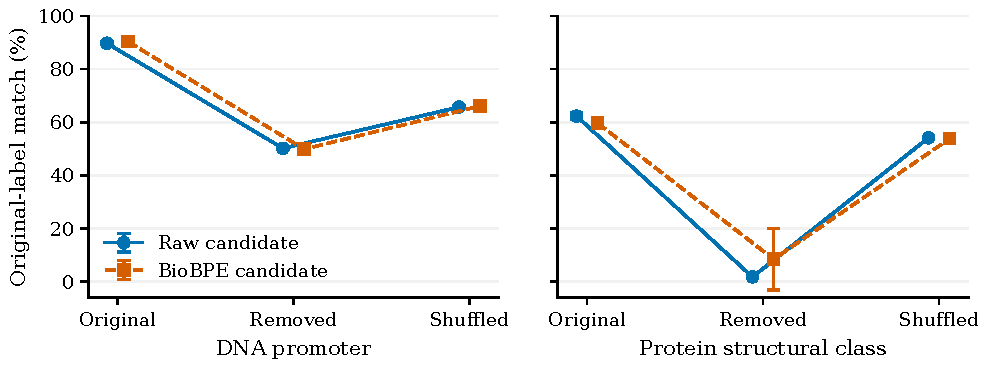
\includegraphics[width=0.91\linewidth]{figures/sequence_diagnostics.pdf}
\caption{Dev sequence-dependence diagnostics. Points and error bars are means and sample SDs across three trained seeds. For shuffled sequences, each seed first averages three deterministic character permutations. The vertical axis measures agreement with the \emph{original} labels: removed or shuffled sequences are interventions, not independently labeled biological examples.}
\label{fig:sequence}
\end{figure}
\paragraph{Sequence dependence.}
The trained text-only control reaches 49.84\% DNA and 29.10\% protein test accuracy, with a constant class prediction within each task/seed. Its low protein macro-F1 reflects the class imbalance. Dev interventions on the sequence-trained \BioBPE{} model reduce original-label matching from 90.34\% to 49.84\% after DNA removal and to 66.12\% after DNA shuffling; protein values change from 59.65\% to 8.42\% and 53.79\%, respectively (Figure~\ref{fig:sequence}). Shuffling preserves character counts but not biological labels. These observations support sequence dependence and residual composition-related signal, without identifying a learned biological mechanism. Inference-time removal is also a distribution shift and must not be equated with the separately trained text-only baseline.

\begin{figure}[t]
\centering
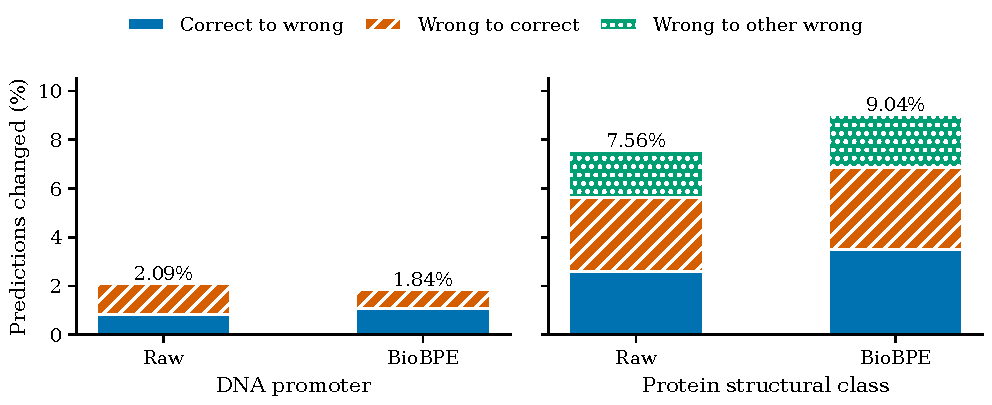
\includegraphics[width=0.91\linewidth]{figures/candidate_order.pdf}
\caption{Dev prediction changes after one deterministic nonidentity candidate permutation per example, with outputs mapped back to canonical labels. Stacks show mean fractions over three seeds. For \BioBPE{} protein predictions, correct-to-wrong and wrong-to-correct changes nearly cancel in accuracy, while wrong-to-other-wrong changes also contribute to instability.}
\label{fig:order}
\end{figure}
\paragraph{Candidate-order sensitivity.}
The same candidate set does not ensure the same prediction. On dev, reordering candidates changes 1.84\% of \BioBPE{} DNA predictions and 9.04\% of protein predictions. For protein, 3.49\% of examples change from correct to wrong, 3.38\% from wrong to correct, and 2.16\% between wrong classes (Figure~\ref{fig:order}; displayed components are rounded). Aggregate accuracy changes by only $-0.11$ percentage points. Raw protein predictions also show sensitivity, with 7.56\% changing. Training with fixed per-example candidate permutations has therefore not produced order invariance. This diagnostic covers one nonidentity permutation per example, not all possible orders, and was not expanded on test.

\section{Limitations}
The evidence concerns two closed-set tasks, one checkpoint, three seeds, and one implemented fixed-head control. Each task has a fixed template and candidate set; no unseen-task, paraphrase, or new-label evaluation was performed. Candidate scoring's measured advantage cannot be assigned solely to textual label semantics because the control changes pooling and input structure. Specialized biological encoders and generative sequence--text systems were not evaluated under a matched budget.

Data independence remains limited. Exact and DNA reverse-complement overlap checks do not establish homology-separated protein evaluation or species-separated DNA evaluation. Historical cluster summaries lack a verified membership mapping to these local records. The biological BPE was fitted on external corpora whose overlap with the benchmark is not fully established, and the parent checkpoint's historical exposure is not excluded. The inherited eligibility filter also restricts coverage. These limitations rule out an unqualified leakage-free generalization claim.

This was an iterative development study, not a publicly preregistered experiment. Earlier compact-vocabulary runs informed development; the final twelve-model protocol was fixed before its test predictions. Seed SDs do not quantify biological sampling uncertainty, and no significance claim is made. The observed order sensitivity and incomplete probability calibration limit direct deployment claims. The study is a computational benchmark, with no experimental or clinical validation.

\section{Conclusion}
Under a fixed supervised budget, a biological-BPE Laya candidate model outperforms the implemented fixed-class and text-only controls on the evaluated short-sequence tasks. Raw candidate input nevertheless gives higher test accuracy, and biological BPE does not improve measured training time. Development diagnostics show that the models use sequence information while remaining sensitive to candidate order. The resulting evidence supports a bounded adaptation baseline and a reliability protocol, rather than a general tokenization benefit or open-ended biological reasoning capability. Further method development requires evaluation designs that address homology and template transfer without reusing this test set for selection.

The data, code, final checkpoints, and historical corpus archive are publicly available at the fixed revisions listed in Appendix~\ref{sec:availability}.

\label{main_end}
\clearpage
\begingroup
\small
\bibliographystyle{plainnat}
\bibliography{references}
\endgroup
\clearpage
\appendix
\section{Reproducibility and complete results}
\paragraph{Versions and artifacts.}
The starting model is \texttt{convaiinnovations/laya-typed-decisions}, revision
\nolinkurl{f9ab0b228f0fc0f14d873dbc99038f135c2da1b2}.
The upstream Laya source revision is
\nolinkurl{573e5b62696ba441230cd6be71d593331b5d23af}.
The initial weight SHA-256 is
\nolinkurl{4fa56de72383a9d3efa9cfa78955733c81b9fc8067a587ca4beb82c78107a24e}.
The final test manifest hashes 288 files and is stored at
\path{artifacts/laya_locked_test/manifest.json}.
Its SHA-256 is
\nolinkurl{9b1594ec0255318ff30486fbea20e3a0172ca1292d1661c040c67800ac86c10e}.
The manifest predates test inference and is checked again after all evaluations. Every checkpoint exactly reproduced its complete dev logits; all test logits were finite. Each model evaluated the same 4,097 sample IDs without truncation. Independent sklearn/SciPy metric recomputation agreed to a maximum absolute error of $2.22\times10^{-16}$.

\paragraph{Data, code, and model availability.}
\label{sec:availability}
The benchmark snapshots, cleaned splits, paper-eligible subsets, frozen manifests, per-example predictions and logits, training/evaluation code, BPE assets, and manuscript materials are publicly available at \href{https://huggingface.co/datasets/dnagpt/laya-bio/tree/0307d5910b0a37f54caecd444241db6b56331701}{\texttt{dnagpt/laya-bio}} (revision \nolinkurl{0307d5910b0a37f54caecd444241db6b56331701}). The default configuration contains 32,050 training, 1,978 selection-dev, 1,986 calibration, and 4,097 test examples; the larger cleaned data are provided separately and are not the paper's evaluation subset.

All twelve final checkpoints (four conditions, three seeds), the original initialization weights, tokenizers, configurations, and loading code are available at \href{https://huggingface.co/dnagpt/laya-bio-models/tree/6d727dd4125d783ab719a35c6b55dd7a69276a8d}{\texttt{dnagpt/laya-bio-models}} (revision \nolinkurl{6d727dd4125d783ab719a35c6b55dd7a69276a8d}; 22.46~GB). Seven historical corpus files and the two actual BPE-training samples are archived at \href{https://huggingface.co/datasets/dnagpt/laya-bio-historical-corpora/tree/bd70a7d157741f8d19ad150adfa350a9b02ba417}{\texttt{dnagpt/laya-bio-historical-corpora}} (revision \nolinkurl{bd70a7d157741f8d19ad150adfa350a9b02ba417}). This archive preserves 106.98~GB of original bytes in 404 lossless Zstandard shards; the 42.55~GB release includes manifests and a SHA-256-verifying restoration script. These historical resources do not imply additional neural continual pretraining in this study.

Release files were checked against remote sizes and content hashes. Anonymous access was verified, including a complete download and restoration of the archived PDB 3Di file. Source declarations and component-specific license terms are preserved; the archive is not assigned a blanket license. Upstream provenance and benchmark overlap remain incompletely resolved, as discussed in the limitations. The released local snapshots, rather than the current BioPAWS-2 page contents, define the experimental data.

\paragraph{Implementation details.}
Input length is capped at 1,024 tokens and the upstream candidate header budget is 256. The original builder's choice instruction is \emph{Choose the correct biological label for the sequence.} The state prefix contains \texttt{Task context:} followed by the cleaned task instruction and \texttt{Sequence:} followed by the sequence. Candidate strings are the canonical class names in Table~\ref{tab:classes}; gold answers are not part of the input. The protein class labels are reproduced as dataset categories, without treating them as a complete structural ontology.

The joint training loop shuffles the combined sample list without class weighting. It uses gradient clipping at norm 1.0, 151 warmup updates, and the final fixed-budget checkpoint. The budget is approximately three passes, but example presentations are reported explicitly because the sampler reshuffles when a full micro-batch no longer fits. AdamW and BF16 settings are shared. Calibration optimizes a single task-specific temperature per checkpoint on the calibration split. Macro metrics retain all two or seven classes; Brier uses the unnormalized sum across classes. ECE15 uses the maximum predicted probability and equal-width bins, including confidence 1 in the final bin.

The historical BPE recipe sampled about 1~GiB each from DNA and protein text using seed 42, with minimum frequency 10. The original vocabulary files, repair details, source scripts, and corpus hashes are preserved. Training observes 18,448 of the 19,999 added DNA tokens and 7,972 of the 8,000 protein tokens. Tokens unobserved in sequences are not claimed to have direct task supervision. The original vocabulary was not retrained on the benchmark.

\begin{table}[ht]
\centering\small
\begin{tabular}{llrrrr}
\toprule
Seed & Model & DNA Acc. & DNA F1 & Protein Acc. & Protein F1 \\
\midrule
20260922 & Raw candidate & 91.14 & 91.14 & 60.55 & 52.56 \\
20260922 & BioBPE candidate & 90.30 & 90.30 & 59.38 & 50.70 \\
20260922 & BioBPE fixed head (B1) & 88.48 & 88.48 & 45.65 & 33.44 \\
20260922 & Text-only candidate & 49.51 & 33.12 & 29.10 & 6.44 \\
20260923 & Raw candidate & 91.42 & 91.42 & 59.94 & 49.72 \\
20260923 & BioBPE candidate & 90.16 & 90.16 & 58.71 & 49.86 \\
20260923 & BioBPE fixed head (B1) & 89.18 & 89.18 & 56.35 & 41.54 \\
20260923 & Text-only candidate & 50.49 & 33.55 & 29.10 & 6.44 \\
20260924 & Raw candidate & 90.72 & 90.72 & 59.43 & 49.61 \\
20260924 & BioBPE candidate & 90.02 & 90.02 & 59.07 & 50.28 \\
20260924 & BioBPE fixed head (B1) & 88.62 & 88.62 & 51.43 & 39.02 \\
20260924 & Text-only candidate & 49.51 & 33.12 & 29.10 & 6.44 \\
\bottomrule
\end{tabular}

\caption{All test seeds; no best-seed selection. Classification metrics are percentages.}
\label{tab:seeds}
\end{table}

\begin{table}[ht]
\centering\scriptsize
\begin{tabular}{llrrrr}
\toprule
Model & Task & Bal. Acc. & MCC & Brier (raw) & ECE (raw) \\
\midrule
Raw candidate & DNA & $91.10 \pm 0.35$ & $0.822 \pm 0.007$ & $0.138 \pm 0.008$ & $0.036 \pm 0.005$ \\
BioBPE candidate & DNA & $90.16 \pm 0.14$ & $0.803 \pm 0.003$ & $0.158 \pm 0.002$ & $0.060 \pm 0.003$ \\
BioBPE fixed head (B1) & DNA & $88.76 \pm 0.37$ & $0.775 \pm 0.007$ & $0.171 \pm 0.002$ & $0.043 \pm 0.014$ \\
Text-only candidate & DNA & $50.00 \pm 0.00$ & $0.000 \pm 0.000$ & $0.500 \pm 0.000$ & $0.006 \pm 0.005$ \\
Raw candidate & Protein & $49.40 \pm 1.81$ & $0.483 \pm 0.007$ & $0.574 \pm 0.011$ & $0.181 \pm 0.000$ \\
BioBPE candidate & Protein & $49.12 \pm 0.81$ & $0.471 \pm 0.004$ & $0.579 \pm 0.003$ & $0.165 \pm 0.005$ \\
BioBPE fixed head (B1) & Protein & $39.50 \pm 4.29$ & $0.370 \pm 0.074$ & $0.620 \pm 0.036$ & $0.049 \pm 0.017$ \\
Text-only candidate & Protein & $14.29 \pm 0.00$ & $0.000 \pm 0.000$ & $0.781 \pm 0.000$ & $0.008 \pm 0.001$ \\
\bottomrule
\end{tabular}

\caption{Additional test metrics, mean $\pm$ sample SD. Balanced accuracy is in percent; MCC, Brier, and ECE are unscaled. Calibrated Brier and ECE are in Table~\ref{tab:calibration}.}
\label{tab:allmetrics}
\end{table}

\begin{table}[ht]
\centering\small
\begin{tabular}{lrrr}
\toprule
Model & Trainable (M) & Training (min) & Peak allocated (GiB) \\
\midrule
Raw candidate & 421.030 & $41.20 \pm 0.90$ & $7.89 \pm 0.00$ \\
BioBPE candidate & 449.701 & $41.24 \pm 0.82$ & $8.41 \pm 0.00$ \\
BioBPE fixed head (B1) & 449.709 & $41.71 \pm 1.01$ & $8.41 \pm 0.00$ \\
Text-only candidate & 449.701 & $40.63 \pm 0.60$ & $8.40 \pm 0.00$ \\
\bottomrule
\end{tabular}

\caption{Measured training cost and trainable parameter counts. Times exclude subsequent evaluation and checkpoint reload checks. Peak allocated memory is the PyTorch training measurement, not the GPU driver's full process footprint. Equal supervision does not imply equal computation.}
\label{tab:resources}
\end{table}

\begin{table}[ht]
\centering\small
\begin{tabular}{llrrr}
\toprule
Task & Representation & Train median & Train p95 & Train max \\
\midrule
DNA & Raw candidate & 174 & 180 & 194 \\
DNA & BioBPE candidate & 93 & 97 & 103 \\
Protein & Raw candidate & 145 & 258 & 318 \\
Protein & BioBPE candidate & 127 & 216 & 282 \\
\bottomrule
\end{tabular}

\caption{Full training-input lengths, including task context and candidates, on the common subset. Values are tokens, not nucleotides or residues.}
\label{tab:lengths}
\end{table}

\begin{table}[ht]
\centering\scriptsize
\begin{tabular}{llrrrr}
\toprule
Model & Task & Original & Removed & Shuffled & Order agreement \\
\midrule
Raw candidate & DNA & $89.73 \pm 0.48$ & $50.16 \pm 0.55$ & $65.67 \pm 0.45$ & $97.91 \pm 0.72$ \\
Raw candidate & Protein & $62.31 \pm 1.41$ & $1.73 \pm 0.00$ & $54.13 \pm 0.54$ & $92.44 \pm 0.19$ \\
BioBPE candidate & DNA & $90.34 \pm 0.05$ & $49.84 \pm 0.55$ & $66.12 \pm 0.31$ & $98.16 \pm 0.62$ \\
BioBPE candidate & Protein & $59.65 \pm 0.87$ & $8.42 \pm 11.60$ & $53.79 \pm 0.64$ & $90.96 \pm 0.51$ \\
\bottomrule
\end{tabular}

\caption{Dev diagnostics (\%). Original is accuracy; removed/shuffled are matching rates against original labels, without assuming intervention-label validity. Order agreement compares semantic predictions after canonicalizing the permutation. Values are mean $\pm$ sample SD.}
\label{tab:diagnostics}
\end{table}

\begin{table}[ht]
\centering\small
\begin{tabular}{lrlr}
\toprule
Task & ID & Canonical class & Test n \\
\midrule
DNA & 0 & Non-promoter & 1062 \\
DNA & 1 & promoter & 1083 \\
Protein & 0 & All Alpha & 328 \\
Protein & 1 & All Beta & 430 \\
Protein & 2 & Alpha and Beta & 568 \\
Protein & 3 & Alpha plus Beta & 456 \\
Protein & 4 & Multi-domain Proteins & 48 \\
Protein & 5 & Mixed Structures & 19 \\
Protein & 6 & Small Proteins and Peptides & 103 \\
\bottomrule
\end{tabular}

\caption{Canonical task classes and eligible test support. The trained text-only protein control predicts class 2 for every example in all three seeds.}
\label{tab:classes}
\end{table}

\paragraph{Development history and test boundary.}
An earlier single-seed experiment used a compact 64-token extension and wrapped sequence pieces, with a frozen-model reference. Those scores are development history and are not mixed into the final raw-input or \BioBPE{} test comparisons. The complete-input list inherited from that stage was held fixed in the later three-seed study. Subsequent experiments used the complete historical BPE and added B1/text-only controls and dev sequence/order diagnostics. The final test included only the four conditions and three seeds listed in Table~\ref{tab:seeds}. No test-dependent perturbation, hyperparameter search, or new training followed this evaluation.

\clearpage
\section{Prospective experiments for the decision-interface claim}
\label{sec:prospective}
\textbf{Status.} This is a follow-up design formulated after the reported test results were inspected. It describes experiments to run, not additional evidence. Existing numbers remain the initial two-task study. New design choices will be fixed using development data, and confirmatory evaluation will require a new, independently held-out biological evaluation set; the old test cannot be presented as a fresh blind test.

\paragraph{Three decision primitives and input arity.}
The completed model evaluates Choice only. A proposed extension follows Jev's three interfaces: \textbf{Choice} assigns a distribution over mutually exclusive labels; \textbf{Noul} returns the probability that a proposition is true; \textbf{Score} assigns probabilities to ordered levels and returns an expected level index. Binary biological tasks fit Noul (or equivalently two-way Choice). Multilabel tasks require a separate Noul probability for each label, allowing multiple positives; they must not use one competing softmax over all labels. A continuous assay can be adapted to Score using training-defined ordered bins and numerical anchors, but this does not make Score an unrestricted native regressor. Original-scale errors, rank correlation, quantization error, and a scalar-regression control are necessary.

Inputs become a list of sequences with explicit modality and role, plus the question and output specification. Protein homology uses two protein sequences; coding correspondence uses a DNA and a protein sequence. Pair boundaries and roles are retained. No paired, Score, or multilabel result is claimed for the existing weights.

\begin{table}[ht]
\centering\small
\begin{tabular}{p{.08\linewidth}p{.36\linewidth}p{.19\linewidth}p{.26\linewidth}}
\toprule
ID & Priority task & Interface / input & Admission status \\
\midrule
C01 & Promoter detection & Noul / DNA & Source pool audited \\
C02 & Splice-site type (3 classes) & Choice / DNA & Source pool audited \\
C03 & TF binding-site detection & Noul / DNA & Source pool audited \\
C04 & Structural class (7 classes) & Choice / protein & Existing study task \\
C05 & Sec versus Tat signal peptide & Choice / protein & Local schema audited \\
C06 & Prokaryotic location (6 classes) & Choice / protein & Local schema audited \\
C07 & Protein homology & Noul / protein pair & Two local views audited \\
C08 & DNA--protein correspondence & Noul / mixed pair & Translation diagnostic \\
C09 & GFP fluorescence & Score / protein & TAPE source verified \\
C10 & Protein stability & Score / protein & TAPE source verified \\
C11 & Multilabel cellular localization & Noul panel / protein & DeepLoc source verified \\
C12 & GO molecular function & Noul panel / protein & DeepGO source verified \\
\bottomrule
\end{tabular}
\caption{Proposed 12-task suite, not completed experiments. Source/schema auditing does not establish homology independence, a frozen new split, or tokenizer eligibility. C08 is a mechanistic consistency diagnostic, not independent evidence of natural biological task breadth.}
\label{tab:planned_tasks}
\end{table}

\paragraph{Sources and scope.}
The added public DNA pools are \path{dnagpt/dna_promoter_300}, \path{dna_splice_site_prediction}, and \path{dna_transcription_factor_prediction}; \path{dnagpt/gene_lan_transfer} supplies coding pairs. TAPE supplies fluorescence and stability tasks \citep{rao2019tape}; DeepLoc 2.0 supplies genuine multilabel localization \citep{thumuluri2022deeploc}; DeepGOZero provides a documented source for function annotation \citep{kulmanov2022deepgozero}. The initial GO design restricts evaluation to 32 training-selected molecular-function terms and must be called GO-MF-Lite, not full GO prediction. Missing GO annotations are not confirmed biological negatives; annotation-recovery conventions and target masks must be specified. The repository catalog records 12 additional views, including DMS effects, enhancer activity, chromatin features, RNA binding preference, and protein interactions. Related windows and synthetic-similarity variants are not independent task families.

\paragraph{Data gates and feasibility.}
The new DNA sources contain one pool named \texttt{train}, including old test members. Those members and their groups must remain isolated. Across local tasks, some localization training sequences also occur in old structural-class and signal-peptide test data, requiring a global registry. Paired examples must be divided by endpoint/parent groups, not random pair rows; exact endpoint separation alone does not prove homology independence. Conflicting labels require quarantine and provenance review. Full-input tokenizer eligibility is especially important for long coding pairs and localization proteins. Standard frame-zero translation exactly separates positive and negative examples in two downloaded coding-pair configurations; it is a mandatory rule baseline and explains why that task is a diagnostic. This is a source audit, not a held-out result.

\paragraph{Three model families.}
The primary comparison will include (i) a sequence encoder with task-specific heads, both independently trained and sharing an encoder; (ii) a sequence--language generator evaluated with free generation, finite-label constrained decoding, and exact candidate likelihood scoring; and (iii) Laya-Bio candidate scoring. The encoder and candidate variants will share initialization, sequence representation, supervision, and trainable-parameter accounting. The three generator interfaces use identical checkpoints and prompts. Cross-architecture comparisons will report pretraining differences, parameter counts, example presentations, and measured cost rather than claim an isolated architectural effect. Raw sequence input is the reference representation; BPE remains a secondary ablation, with both prior representations retained in the historical results.

\paragraph{Block 1: label validity and biological accuracy.}
On the same examples and candidate sets, separately report (a) exact output-contract violations, (b) unambiguous canonical-label mapping failures, and (c) wrong in-set predictions. A frozen alias dictionary may recognize a harmless synonym in analysis, but must not erase its strict contract violation. Exact string-to-ID mapping, not an LLM judge, defines validity. Invalid, ambiguous, truncated, and failed responses count against end-to-end accuracy and macro-F1; conditional accuracy among valid outputs is secondary. Fixed heads and completed constrained decoders should also have zero out-of-set labels. Any advantage beyond validity must therefore appear in predictive quality, reusable task handling, calibration, or measured cost. For probabilistic systems, evaluate NLL/Brier and calibration independently of prose confidence claims. Binary tasks additionally require AUROC/AUPRC and MCC; multilabel tasks require micro/macro-AUPRC and frozen-threshold F1; Score tasks require original-scale MAE/RMSE and Spearman. Do not average these heterogeneous metrics into an overall accuracy. Shared-head controls must include sigmoid multilabel and scalar-regression outputs.

\paragraph{Block 2: shared task handling and transfer.}
Use the proposed suite to include several tasks in each sequence modality; where available, ask different labeled questions about the same sequence. This removes modality as a sufficient task selector. Compare joint versus single-task training under the same per-task exposure, and compare shared candidate scoring against the shared-encoder multihead control. Train separate leave-one-task-out variants for localization (C06) and stability (C10): exclude C11 as well for strict localization-family transfer. No held-out-task supervision or calibration is allowed; Score levels and anchors require an external specification independent of held-out targets. A model jointly trained on all 12 tasks is not zero-shot on any of them. Report zero-shot candidate/generator results separately from fixed-head few-shot adaptation, for which a new head is required. Report a new-task learning curve if sample-efficient adaptation is claimed. If only trained tasks work, retain the narrower shared-supervision claim.

\paragraph{Block 3: label identity versus semantic stability.}
Predefine meaning-preserving question paraphrases, verified label aliases/descriptions, and candidate permutations. Return opaque candidate IDs while presenting descriptions; randomize the ID-to-description association per example to prevent fixed output-coordinate shortcuts. A no-description version tests reliance on label meaning. These interventions must preserve gold semantic labels through explicit mappings. Report validity and accuracy for each variant, canonicalized prediction agreement, and the change in probabilities. A valid but changed or wrong answer is semantic instability, not an out-of-set error. Missing-gold candidates form a separate open-set stress test requiring an explicit abstention policy; they must not be included as ordinary closed-set errors with an unavailable target.

\paragraph{Block 4: operational cost and uncertainty.}
Measure batch-1 median and 95th-percentile latency, fixed-batch throughput, and peak GPU memory on the same hardware, including tokenization, label constraints, and output parsing. For multilabel tasks, measure the entire label panel, including repeated sequence encodings and any chunking; one binary call is not a full-panel prediction. Freeze warm-up, input-length bins, candidate counts, output-length limits, and repetition counts before timing. Report model compute separately from network latency if a hosted baseline is used. Fit calibration only on the calibration split. Probability quality and accuracy must accompany timing: a fast but inaccurate or poorly calibrated decision model does not establish a useful advantage. No latency superiority is claimed from the present training-time measurements.

\paragraph{Execution boundary.}
Run definitions and gates are in \path{refine-logs/EXPERIMENT_PLAN.md} and \path{refine-logs/EXPERIMENT_TRACKER.md}. A six-task pilot (C01/C02/C04/C07/C09/C11) precedes admission of the full suite and a measured compute estimate. The main plan has 21 fits: three joint model families and four independent-task anchors, each over three seeds. Two leave-one-task-out settings add 12 candidate/generator fits. These transfer tests are required before unseen-task claims.

\end{document}
